
\usepackage[T1]{fontenc}
\usepackage[utf8]{inputenc}

% Usado pela Ficha catalográfica
\usepackage{lastpage} 

% Controle das cores
\usepackage{color} 

% Inclusão de gráficos
\usepackage{graphicx} 

%Posicionamento de figuras [!htb]
\usepackage{float} 

% Para melhorias de justificação
\usepackage{microtype}  

\usepackage[colorinlistoftodos]{todonotes}



% Para importar arquivos tex de outros diretórios.
\usepackage{import} 

% Usado para figuras lado a lado / subfigure.
\usepackage{subcaption} 

% Usado para pegar o papel milimetrado para graficos.
\usepackage{pdfpages}

% Usado para o papel milimetrado.
\usepackage{tikz} 

% Cancel em equations.
\usepackage[makeroom]{cancel} 

% Usado para marca dagua (water mark).
\usepackage{eso-pic} 

%Usado para espaço de anotações (quadro/caixa).
\usepackage[most]{tcolorbox} 

%Tabela: várias linhas em uma célula.
\usepackage{multirow} 


% Indenta o primeiro parágrafo de cada seção.
\usepackage{indentfirst} 


% ---
% Pacotes de citações
% ---

% Paginas com as citações na bibl
\usepackage[brazilian,hyperpageref]{backref} 

%\usepackage[alf]{abntex2cite}	% Citações padrão ABNT - alfabetico
\usepackage[num]{abntex2cite}	% Citações padrão ABNT - numérico
\citebrackets[] % Citação em brakets
% ---


% ---
% Pacotes adicionais, usados apenas no âmbito do Modelo Canônico do abnteX2
% ---
\usepackage{lipsum}	 % para geração de dummy text
\usepackage{amsmath}
\usepackage{amsbsy} % para ambiente matemático
\usepackage{latexsym}
\usepackage{amssymb}
\usepackage{ifsym}
%\usepackage{ulem}
% ---



% --- 
% CONFIGURAÇÕES DE PACOTES
% --- 

% O tamanho do parágrafo.
\setlength{\parindent}{1.3cm}

% Controle do espaçamento entre um parágrafo e outro.
% Tente também \onelineskip.
\setlength{\parskip}{0.2cm}  


% Configuração da marca d'água (definir arquivo de imagem)
% Necessário: "\usepackage{eso-pic}"
\newcommand\BackgroundPic{
\put(0,0){
\parbox[b][\paperheight]{\paperwidth}{%
\vfill
\centering

\includegraphics[width=\paperwidth,height=\paperheight,
keepaspectratio]{images/UNIFOR_WM1.eps}%Water Mark
\vfill
}}}


% Caixa de "anotações" para os alunos.
% Necessário "\usepackage[most]{tcolorbox}"
\newcommand{\anotacoes}[1]{
\begin{tcolorbox}[breakable,
enhanced jigsaw,
fonttitle=\bfseries,
%title=Anotações,
opacityframe=0.5, opacityback=0.25, opacitybacktitle=0.25, opacitytext=0.8,
%colback=red!5!white, colframe=red!75!black, colbacktitle=yellow!20!red,
width=\linewidth+0.5cm,
enlarge left by=-0.5cm
]
\begin{minipage}[t][#1][t]{\linewidth}
\end{minipage}
\end{tcolorbox}
}


% Papel milimetrada (metade de uma folha)
% Necessário "\usepackage{tikz}"
\newcommand{\papelmilimetrado}{
\noindent \hspace{-0.9cm}
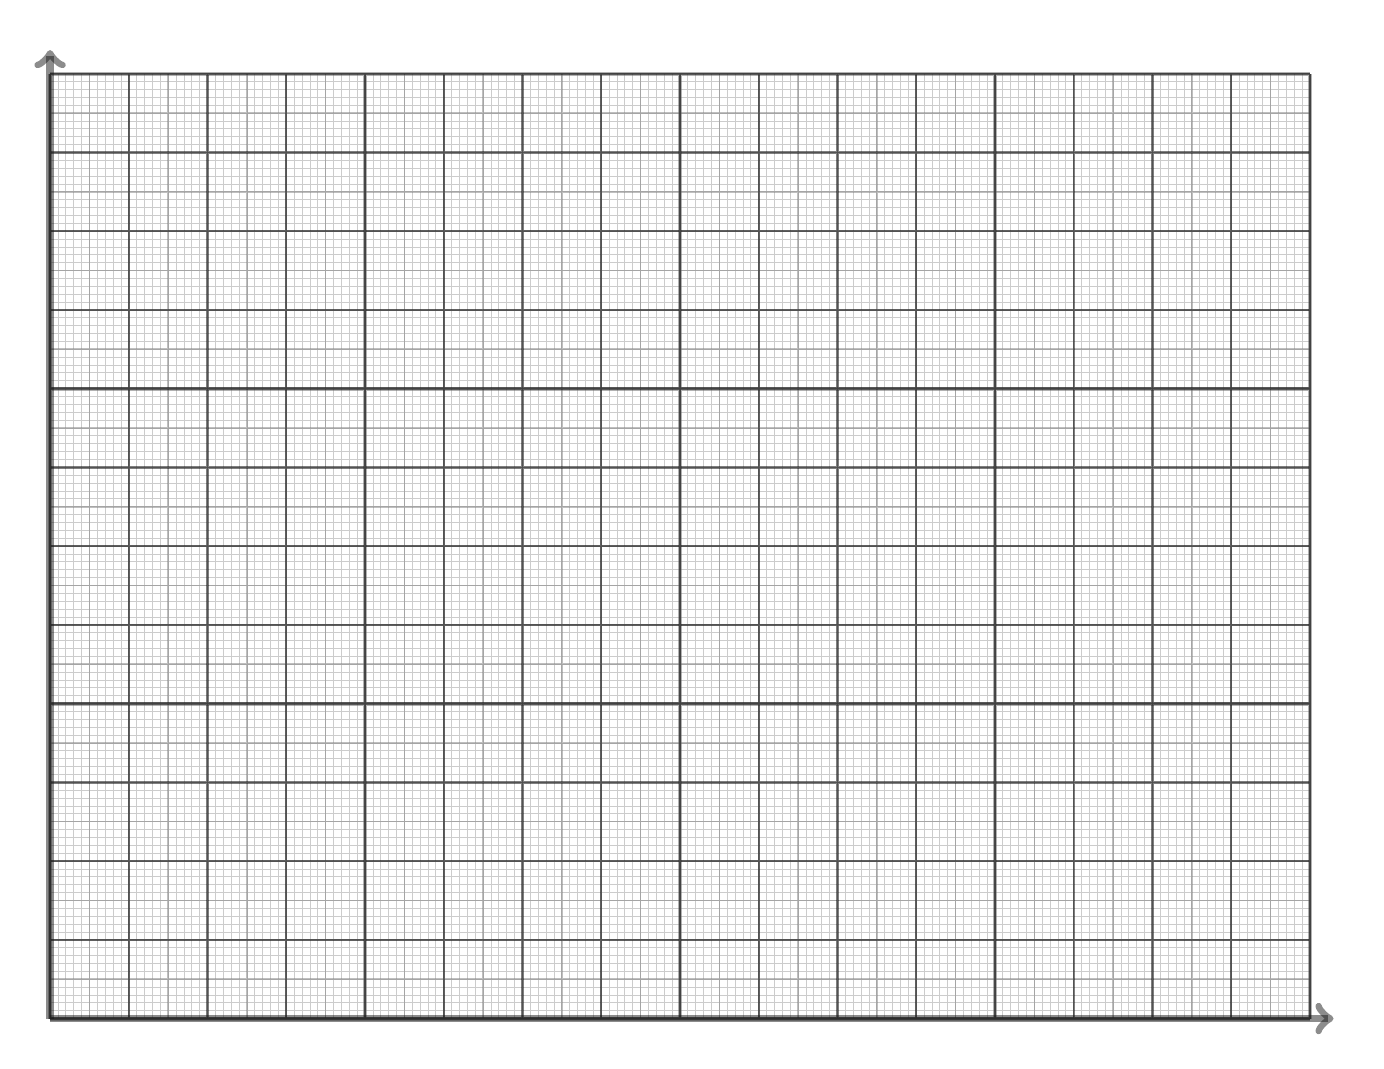
\begin{tikzpicture}[x=1cm, y=1cm,semitransparent]
\draw[step=1mm, line width=0.1mm, black!40!white] (0,0) grid (16,12);
\draw[step=5mm, line width=0.2mm, black!50!white] (0,0) grid (16,12);
\draw[step=4cm, line width=0.5mm, black!60!white] (0,0) grid (16,12);
\draw[step=1cm, line width=0.3mm, black!100!white] (0,0) grid (16,12);
\draw[thick,->,line width=1mm,black!90!white] (0,0) -- (16.3,0) node[anchor=north west] {};
\draw[thick,->,line width=1mm,black!90!white] (0,0) -- (0,12.3) node[anchor=south east] {};
\end{tikzpicture}
}


% ---
% Configurações de aparência do PDF final
% ---

% alterando o aspecto da cor azul
\definecolor{blue}{RGB}{41,5,195}

% informações do PDF
\makeatletter
\hypersetup{
     	%pagebackref=true,
		pdftitle={\@title}, 
		pdfauthor={\@author},
    	pdfsubject={\imprimirpreambulo},
	    pdfcreator={LaTeX with abnTeX2},
		pdfkeywords={física}{experimentos}{prática}{laboratório}, 
		colorlinks=true,       		% false: boxed links; true: colored links
    	linkcolor=black,          	% color of internal links, Ex: blue
    	citecolor=black,        		% color of links to bibliography, Ex: blue
    	filecolor=black,      		% color of file links, Ex: magenta
		urlcolor=black,		%Ex: blue
		bookmarksdepth=4
}
\makeatother
% --- 


%== Gerar/Inserir o indice
\makeindex

